\documentclass{beamer}
\usepackage{amsmath}
%\usepackage{enumitem}
\usepackage{graphicx}
\usepackage{pdflscape}
\usepackage{float}
\usepackage{multirow}

\usetheme{Dresden}

%\setbeamertemplate{itemize body begin}{\tiny}
%\setbeamertemplate{itemize items}[triangle]


\begin{document}

\title{A multi-view Automatic Lip-reading}
\subtitle{Group 12, The Kip-reader's}
\author{Houjeung Han \and Jesper Loenbaek \and Youngsoo Jang}
\institute%
{
    School of Computing\\
    KAIST\\
    Daejeon, Korea
}

\date{5-19 Dec 2016}
\frame{\titlepage}

\begin{frame}{Content}
    \begin{itemize}
        \item About Lip-reading
        \item Automatic Lip-reading and its application
        \item General approach and challenges
        \item Experimental setup and database
        \item Baseline architecture
        \item Our approach
        \item Result 
        \item Conclusion 
    \end{itemize}
    \vspace{0.5cm}
    \begin{columns}[T]
    \column{.5\textwidth}
    \column{.5\textwidth}
    \end{columns}
\end{frame}

\begin{frame}{About Lip-reading}
    \begin{itemize}
        \item What is Lip-reading?
        \begin{itemize}
            \item Understanding speech by visually interpreting movement of lips, face and tongue
        \end{itemize}
    \end{itemize}
    \begin{itemize}
        \item Who use it?
        \begin{itemize}
            \item Deaf or head-of-hearing people
            \item People with normal hearing process (McGurk Effect)
        \end{itemize}
    \end{itemize}
\end{frame}

\begin{frame}{Automatic Lip-reading}
    \begin{itemize}
        \item Understand speech from a video stream
        \begin{itemize}
            \item Input: sequence of images
            \item Output: text 
        \end{itemize}
    \end{itemize}
    \begin{center}
    \includegraphics[width=0.8\textwidth]{fig/automaticLipreadingArchi.pdf}   
    \end{center}
\end{frame}

\begin{frame}{Application}
    \begin{itemize}
        \item Enhancing speech recognition
        \begin{itemize}
            \item Combining audio and visual speech recognition 
        \end{itemize}
        \item Visual Password 
        \item Silent speech interface
        \item Forensic video analysis 
    \end{itemize}
\end{frame}

\begin{frame}{General Approach}
    \begin{itemize}
        \item Extract features from individual images
        %\begin{itemize}
        %    \item Different mouth shape
        %\end{itemize}
        \item Correlate features in time
        %\begin{itemize}
        %    \item Difference in visual pronunciation
        %\end{itemize}
        \item Classification 
    \end{itemize}
    \begin{center}
    \includegraphics[width=0.9\textwidth]{fig/alrVisualTempClass.pdf}   
    \end{center}
\end{frame}

\begin{frame}{Challenges}
    \begin{itemize}
        \item Personal dependencies
        \begin{itemize}
            \item Mouth shape 
            \item Visual pronunciation  
        \end{itemize}
        \item Recording dependencies 
        \begin{itemize}
            \item Change in illumination 
            \item Camera angle
        \end{itemize}
    \end{itemize}
\end{frame}

\begin{frame}{Experimental Setup}
    \begin{itemize}
        \item Speaker dependent
        \begin{itemize}
        \item One person is used for training and testing
        \end{itemize}
        \item Speaker independent
        \begin{itemize}
        \item Different people is used for training and testing
        \end{itemize}
    \end{itemize}
    \begin{itemize}
        \item Single-view 
        \begin{itemize}
        \item Same view used for training and testing
        \end{itemize}
        \item Cross-view 
        \begin{itemize}
        \item One view used for training, other used for testing
        \end{itemize}
        \item Multi-view 
        \begin{itemize}
        \item Multiple-view used for training and testing
        \end{itemize}
    \end{itemize}
    \begin{center}
    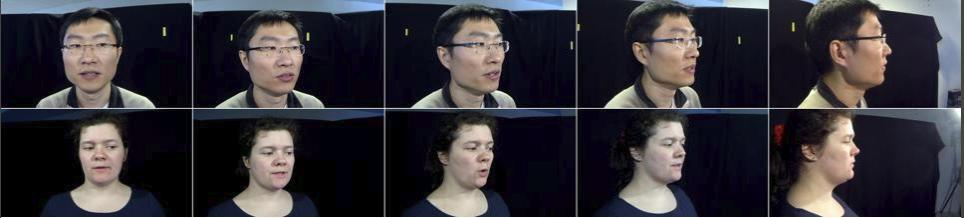
\includegraphics[width=\textwidth]{fig/ouluFullView.jpg}   
    \end{center}
\end{frame}

\begin{frame}{Experimental Setup}
    \begin{itemize}
        \item Speaker dependent
        \begin{itemize}
        \item One person is used for training and testing
        \end{itemize}
        \item \alert{Speaker independent}
        \begin{itemize}
        \item Different people is used for training and testing
        \end{itemize}
    \end{itemize}
    \begin{itemize}
        \item \alert{Single-view}
        \begin{itemize}
        \item Same view used for training and testing
        \end{itemize}
        \item \alert{Cross-view}
        \begin{itemize}
        \item One view used for training, other used for testing
        \end{itemize}
        \item \alert{Multi-view}
        \begin{itemize}
        \item Multiple-view used for training and testing
        \end{itemize}
    \end{itemize}
    \begin{center}
    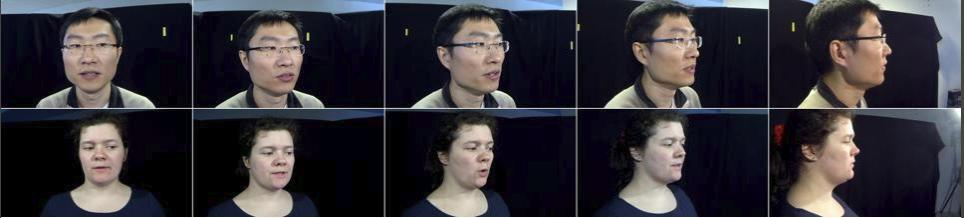
\includegraphics[width=\textwidth]{fig/ouluFullView.jpg}   
    \end{center}
\end{frame}

\begin{frame}{Dataset}
    \begin{columns}[T]
    \column{.65\textwidth}
        \begin{itemize}
            \item Lip-reading challenge (MLAC 2016)%\footnote{http://ouluvs2.cse.oulu.fi/ACCVE.html} (MLAC 2016)
            \item OuluVS2 database\cite{Anina2015} 
        \end{itemize}
        \begin{itemize}
            \item Recording
            \begin{itemize}
                \item \textbf{52} subjects
                \item \textbf{five} camera angles 
            \end{itemize}
            \item Content 
        \end{itemize}
    \column{.35\textwidth}
        \begin{center}
        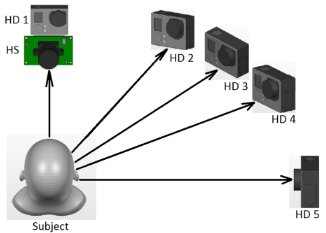
\includegraphics[width=\textwidth]{fig/ouluMultiView.jpg}   
        \end{center}
    \end{columns}
    \begin{center}
    \footnotesize
    \begin{tabular}{l|p{5cm}}
        \multirow{2}{*}{Digits}  
        & "1 7 3 5 1 6 2 6 6 7"\\
        & "4 0 2 9 1 8 5 9 0 4"\\
        \hline
        \multirow{2}{*}{Phrases}  
        & "Thank you"\\
        & "Have a good time"\\
        \hline
        TIMIT & "Chocolate and roses never fail as a romantic gift"
    \end{tabular}
    \end{center}
    %\begin{center}
    %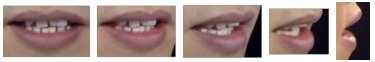
\includegraphics[width=0.8\textwidth]{fig/ouluPreprocessed.jpg}   
    %\end{center}
\end{frame}

\begin{frame}{Baseline}
    \begin{itemize}
        \item End-to-End neural network
        \item Visual model: Convolutional Neural Network (CNN)
        \item Temporal model: Long Short-Term Memory (LSTM)
        \item Classifier: Support Vector Machine (SVM)
    \end{itemize}
    \begin{center}
    \includegraphics[width=0.8\textwidth]{fig/baseline.pdf}   
    \end{center}
\end{frame}

\begin{frame}{Our Approach}
    \begin{itemize}
        \item Try different visual and temporal models
    \end{itemize}
    \begin{center}
    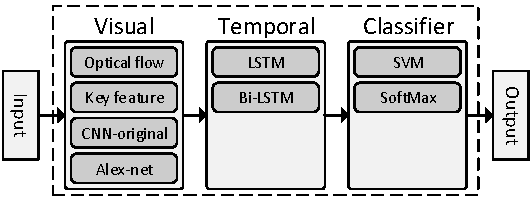
\includegraphics[width=0.8\textwidth]{fig/highLevelArchitecture.pdf}   
    \end{center}
\end{frame}

\begin{frame}{Visual Models}
    \begin{columns}[T]
    \column{.5\textwidth}
    \begin{itemize}
        \item CNN-baseline
        \begin{figure}
        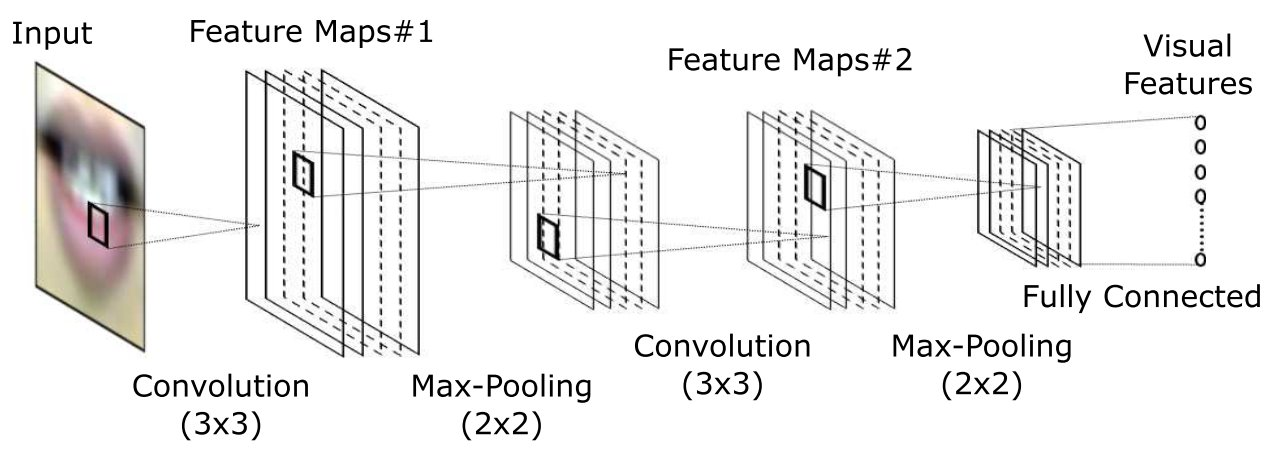
\includegraphics[width=.9\textwidth]{fig/cnnOriginal.jpg}   
        \end{figure}
    \end{itemize}
    \column{.5\textwidth}
    \begin{itemize}
        \item Alex-net 
        \begin{figure}
        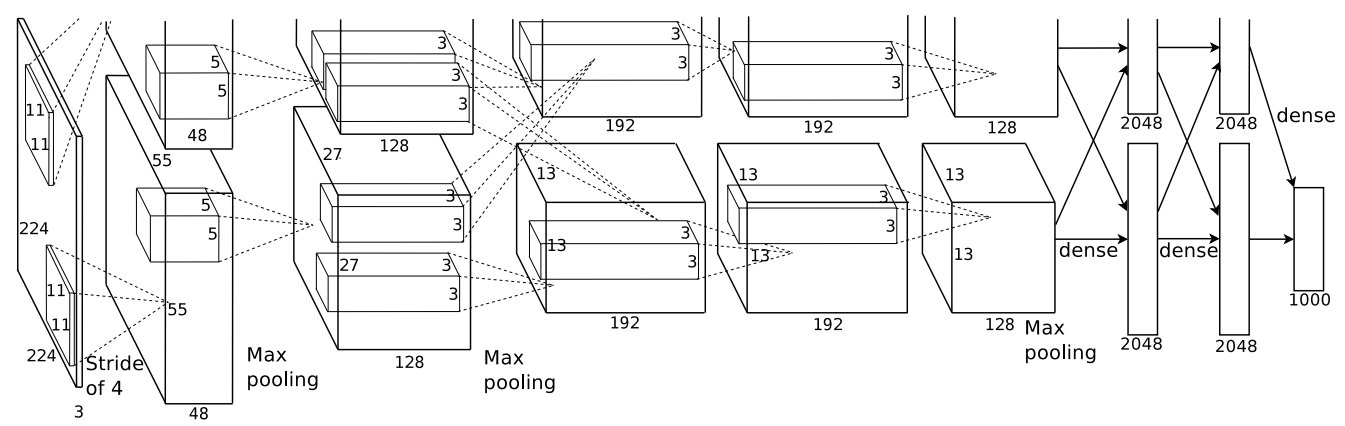
\includegraphics[width=.9\textwidth]{fig/alexNet.jpg}   
        \end{figure}
    \end{itemize}
    \end{columns}
    \begin{columns}[T]
    \column{.5\textwidth}
    \begin{itemize}
        \item Key features 
        \begin{figure}
        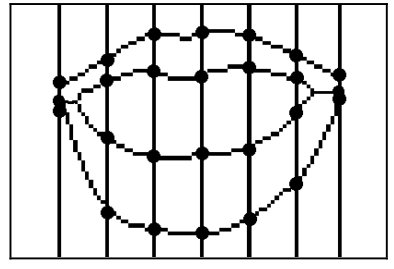
\includegraphics[width=.5\textwidth]{fig/keyFeature.jpg}   
        \end{figure}
    \end{itemize}
    \column{.5\textwidth}
    \begin{itemize}
        \item Optical flow
        %\begin{figure}
        %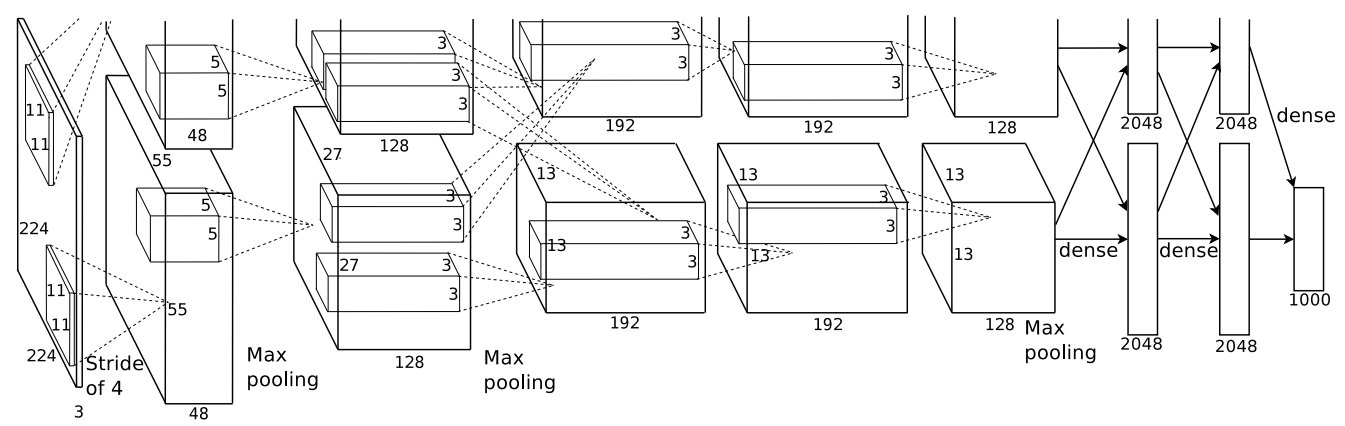
\includegraphics[width=.9\textwidth]{fig/alexNet.jpg}   
        %\end{figure}
    \end{itemize}
    \end{columns}
\end{frame}

\begin{frame}{Temporal Models}
    \begin{itemize}
        \item Long Short-Term Memory 
        %\begin{figure}
        %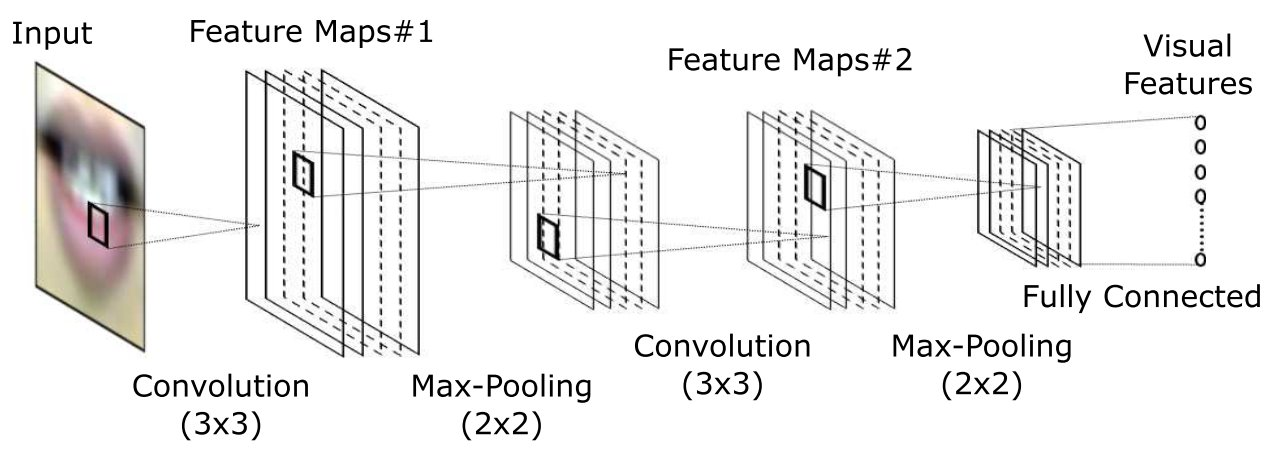
\includegraphics[width=.9\textwidth]{fig/cnnOriginal.jpg}   
        %\end{figure}
    \end{itemize}
    \begin{itemize}
        \item Bidirectional Long Short-Term memory 
        %\begin{figure}
        %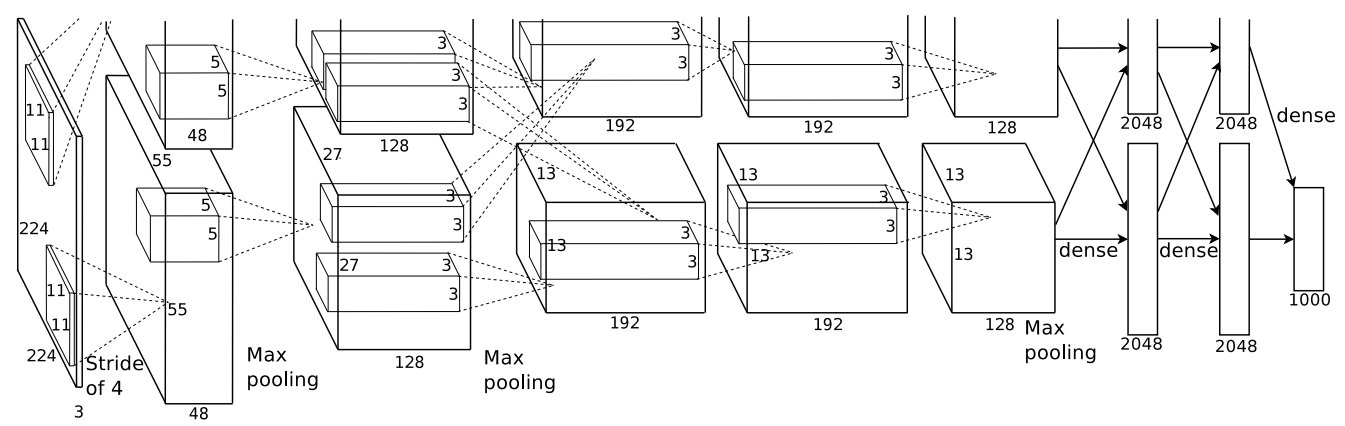
\includegraphics[width=.9\textwidth]{fig/alexNet.jpg}   
        %\end{figure}
    \end{itemize}
\end{frame}

\begin{frame}{Results}
\end{frame}

\begin{frame}{Conclusion}
\end{frame}

\bibliographystyle{plain}
 %argument is your BibTeX string definitions and bibliography database(s)
\bibliography{tmp,mendeley}

\end{document}
